% 定义颜色：由浅入深体现规模增长
\definecolor{color_base}{RGB}{180, 180, 180} % 灰色：原始查询
\definecolor{color_3b}{RGB}{198, 219, 239}
\definecolor{color_7b}{RGB}{158, 202, 225}
\definecolor{color_14b}{RGB}{107, 174, 214}
\definecolor{color_32b}{RGB}{49, 130, 189}
\definecolor{color_72b}{RGB}{8, 81, 156}

% % 替换原有的颜色定义
% \definecolor{color_base}{RGB}{200, 200, 200} % 极浅灰
% \definecolor{color_3b}{RGB}{237, 248, 251}   % 极淡青
% \definecolor{color_7b}{RGB}{179, 205, 227}   % 灰蓝
% \definecolor{color_14b}{RGB}{140, 150, 198}  % 紫蓝
% \definecolor{color_32b}{RGB}{136, 65, 157}   % 深紫
% \definecolor{color_72b}{RGB}{77, 0, 75}      % 极深紫

% % 替换原有的颜色定义
% \definecolor{color_base}{RGB}{100, 100, 100} % 灰色
% \definecolor{color_3b}{RGB}{68, 1, 84}       % 紫色
% \definecolor{color_7b}{RGB}{59, 82, 139}     % 靛蓝
% \definecolor{color_14b}{RGB}{33, 145, 140}    % 青色
% \definecolor{color_32b}{RGB}{94, 201, 98}    % 嫩绿
% \definecolor{color_72b}{RGB}{253, 231, 37}   % 明黄（突出最强性能）
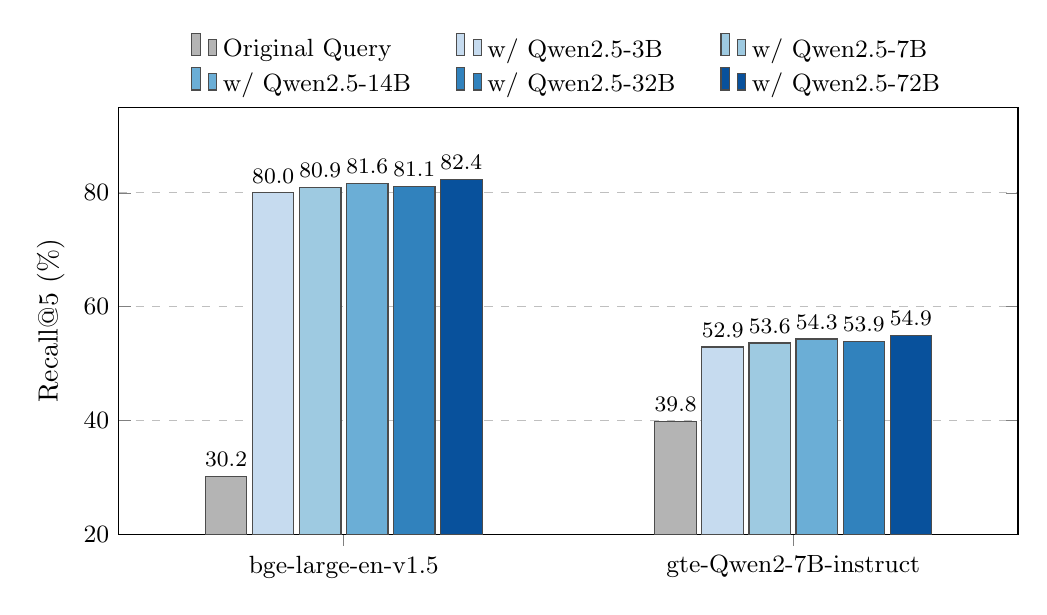
\begin{tikzpicture}
\begin{axis}[
    ybar,
    bar width=15pt, % 柱子宽度
    width=13cm,
    height=7cm,
    enlarge x limits=0.5,
    ylabel={Recall@5 (\%)},
    symbolic x coords={bge-large-en-v1.5, gte-Qwen2-7B-instruct},
    xtick=data,
    tick label style={font=\small},
    ymin=20, ymax=95,
    ymajorgrids=true,
    grid style=dashed,
    legend style={
        at={(0.5, 1.0)}, % 图例置于上方
        anchor=south,
        legend columns=3,
        font=\small,
        draw=none,
        /tikz/every even column/.append style={column sep=0.5cm}
    },
    legend cell align=left,
    nodes near coords, % 在柱子上方显示数值
    % every node near coord/.append style={font=\tiny, rotate=90, anchor=west, /pgf/number format/fixed, /pgf/number format/precision=1}
    every node near coord/.append style={font=\footnotesize, /pgf/number format/fixed zerofill, /pgf/number format/precision=1}
]

% 1. 原始查询 (Baseline) - 对应文中“低基线分数”
\addplot[fill=color_base, draw=black!70] coordinates {
    (bge-large-en-v1.5, 30.2) 
    (gte-Qwen2-7B-instruct, 39.8)
};

% 2. Qwen2.5-3B 重写 - 对应文中“显著性能跃升”的第一步
\addplot[fill=color_3b, draw=black!70] coordinates {
    (bge-large-en-v1.5, 80.0) 
    (gte-Qwen2-7B-instruct, 52.9)
};

% 3. Qwen2.5-7B
\addplot[fill=color_7b, draw=black!70] coordinates {
    (bge-large-en-v1.5, 80.9) 
    (gte-Qwen2-7B-instruct, 53.6)
};

% 4. Qwen2.5-14B
\addplot[fill=color_14b, draw=black!70] coordinates {
    (bge-large-en-v1.5, 81.6) 
    (gte-Qwen2-7B-instruct, 54.3)
};

% 5. Qwen2.5-32B
\addplot[fill=color_32b, draw=black!70] coordinates {
    (bge-large-en-v1.5, 81.1) 
    (gte-Qwen2-7B-instruct, 53.9)
};

% 6. Qwen2.5-72B - 对应文中“性能逼近理论上限”
\addplot[fill=color_72b, draw=black!70] coordinates {
    (bge-large-en-v1.5, 82.4) 
    (gte-Qwen2-7B-instruct, 54.9)
};

\legend{Original Query, w/ Qwen2.5-3B, w/ Qwen2.5-7B, w/ Qwen2.5-14B, w/ Qwen2.5-32B, w/ Qwen2.5-72B}

\end{axis}
\end{tikzpicture}